%!TeX root = ../My_thesis.tex


% @inproceedings{my-dataset,
%     title = "Crowdsourced Corpus of Sentence Simplification with Core Vocabulary",
%     author = "Katsuta, Akihiro  and
%       Yamamoto, Kazuhide",
%     booktitle = "Proceedings of the Eleventh International Conference on Language Resources and Evaluation ({LREC} 2018)",
%     month = may,
%     year = "2018",
%     address = "Miyazaki, Japan",
%     publisher = "European Language Resources Association (ELRA)",
%     url = "https://www.aclweb.org/anthology/L18-1072",
% }


% .---|||___|||--- C H A P T E R ---|||___|||---. %
\chapter{Детали практической реализации}
% .---|||___|||--- C H A P T E R ---|||___|||---. %


% .---|||___|||--- S E C T I O N ---|||___|||---. %
\section{Инструменты и исходный код}
% .---|||___|||--- S E C T I O N ---|||___|||---. %


% .---|||___|||--- S U B S E C T I O N ---|||___|||---. %
\subsection{Выбор инструментов для системы упрощения}
% .---|||___|||--- S U B S E C T I O N ---|||___|||---. %


В данной работе используются следующие инструменты:
\begin{enumerate}[1.]%
  \item Машинное обучение. Для обучения модели будет использоваться Python в связке с фреймворком для машинного обучения PyTorch~\cite{PyTorch}, предоставляющий широкие возможности для реализации нейронных сетей, в том числе, там присутствует поддержка ранее упомянутых Transformer'ов.
  \item Токенизация. Для токенизации японского текста будет использоваться библиотека MeCab~\cite{MeCab} (он также вычисляет части речи токенов).
  \item Эмбеддинги. Готовые модели с эмбеддингами могут быть взяты из Python-библиотеки Spacy~\cite{Spacy} (в том числе там есть эмбеддинги для японского языка).
  \item Сервер. Тут, опять же, будет использован Python с фреймворком Falcon~\cite{Falcon}, позволяющим создавать легковесный back-end. То есть будет реализован REST API сервер.
  \item Веб-приложение. Будет использоваться TypeScript~\cite{TypeScript} с библиотекой Lit~\cite{Lit} (библиотека для веб-компонентов).
\end{enumerate}

Система будет доступна в браузере в виде простого веб-приложения, то есть модель будет обучена на Python, а пользоваться обученной моделью можно будет в любом современном браузере (пользователю ничего не нужно будет устанавливать).


% .---|||___|||--- S U B S E C T I O N ---|||___|||---. %
\subsection{Объяснение выбранной архитектуры}
% .---|||___|||--- S U B S E C T I O N ---|||___|||---. %


Описанная архитектура «приложение-сервер» выбрана неслучайно. Дело в том, что в отличие, к примеру, от настольного приложения, пользователю ничего не нужно скачивать "--- он просто открывает веб-приложение и может пользоваться приложением. Обученная модель используется на сервере, что позволяет её чаще обновлять, а возможно даже и заменить на более удачную.

Это также может позволить другим разработчикам взять готовую часть решения "--- например, взять уже существующее приложение и использовать там свою модель для упрощения. Или же, наоборот, использовать в своём существующем приложении сервер, представленный в данной работе, просто делая к нему запрос по ранее упомянутому пути (так как сервер не имеет привязки к приложению, сделать это довольно просто, нужно лишь настроить домены, которым будет дан доступ к серверу).


% .---|||___|||--- S U B S E C T I O N ---|||___|||---. %
\subsection{Исходный код системы}
% .---|||___|||--- S U B S E C T I O N ---|||___|||---. %


Исходный код разработанной системы был размещён в 2-х репозиториях на GitHub:
\begin{itemize}%
  \item приложение можно найти в репозитории~\cite{AppGithub},
  \item модель с сервером "--- в репозитории~\cite{ServerGithub}.
\end{itemize}

Разделение на 2 репозитория было сделано затем, чтобы обновление одного из компонентов (сервер/приложение) не затрагивало другой компонет системы.
К примеру, если кто-то будет использовать сервер с упрощением, то ему вовсе не обязательно знать о том, что обновилось пользовательское приложение (которым он, возможно, и вовсе не пользуется).


% .---|||___|||--- S E C T I O N ---|||___|||---. %
\section{Как устроен Transformer изнутри}
% .---|||___|||--- S E C T I O N ---|||___|||---. %


Для ускорения вычислений в PyTorch используются не матрицы размерности~$N \times M$, а тензоры размерности~$B \times M \times N$ (где $B$ "--- размер батча), то есть матрицы обрабатываются батчами размера~$B$. Ускорение происходит за счёт оптимизированного вычисления батчей на видеокартах в PyTorch. Однако для простоты изложения будем считать, что работаем мы с матрицами.


% .---|||___|||--- S U B S E C T I O N ---|||___|||---. %
\subsection{Механизм внимания}
% .---|||___|||--- S U B S E C T I O N ---|||___|||---. %


Вернёмся к формуле~\eqref{scaled-dot-product-attention}. Программно её можно реализовать следующим образом:

\begin{minted}[tabsize=2, mathescape, linenos, xleftmargin=20pt, fontsize=\scriptsize]{python}
def scaledDotProductAttention(
  query: Tensor,
  key: Tensor,
  value: Tensor,
  mask: Optional[Tensor] = None
) -> Tensor:
  # Считаем scale, на который будем делить
  scale = query.size(-1) ** 0.5
  # Перемножаем матрицы query и key, делим их на scale
  temp = query.bmm(key.transpose(1, 2)) / scale

  # Применяем маску, если она есть
  if (mask is not None):
    temp += mask

  # Применяем softmax к измерению embedding'ов
  softmax = f.softmax(temp, dim=-1)
  # Перемножаем softmax с матрицей value
  return softmax.bmm(value)
\end{minted}

Обратим внимание на то, что в коде используется некая маска. О том, что это и зачем она нужна, поговорим в следующем разделе.


% .---|||___|||--- S U B S E C T I O N ---|||___|||---. %
\subsection{Маска в механизме внимания}
% .---|||___|||--- S U B S E C T I O N ---|||___|||---. %


Как же выглядит маска? Просто создаётся треугольная матрица формы $ \text{size} \times \text{size} $, в левой части которой «$0$», а в правой "--- «$-\infty$». Нужно это для того, чтобы при обучении не показывать полностью переведённые (упрощённые) предложения модели (защита от переобучения). То есть «$-\infty$» при суммировании маски со scores заставляет модель «принебречь» частями предложения. Матрица имеет следующий вид (см.~\firef{mask-matrix}).

\begin{equation}\label{mask-matrix}%
  \begin{bmatrix}
    0 & -\infty & -\infty & \ldots & -\infty & -\infty \\
    0 & 0 & -\infty & \ldots & -\infty & -\infty \\ 
    \ldots & \ldots & \ldots & \ldots & \ldots & \ldots \\ 
    0 & 0 & 0 & \ldots & -\infty & -\infty \\ 
    0 & 0 & 0 & \ldots & 0 & -\infty \\ 
    0 & 0 & 0 & \ldots & 0 & 0 \\ 
  \end{bmatrix}_{\text{\texttt{size}} \times \text{\texttt{size}}}  
\end{equation}

Например, матрица маски размера $ 4\times4 $ представлена на~\firef{mask-matrix-example}.

\begin{equation}\label{mask-matrix-example}%
  \begin{bmatrix}
    0 & -\infty & -\infty & -\infty \\
    0 & 0 & -\infty & -\infty \\ 
    0 & 0 & 0 & -\infty \\ 
    0 & 0 & 0 & 0 \\ 
  \end{bmatrix}  
\end{equation}

Реализовать создание такой матрицы довольно несложно, в PyTorch это можно сделать следующим образом:

\begin{minted}[tabsize=2, mathescape, linenos, xleftmargin=20pt, fontsize=\scriptsize]{python}
def generateSquareSubsequentMask(size: int, device: torch.device) -> Tensor:
  # Создаём треугольную матрицу
  mask = (torch.triu(torch.ones((size, size), device=device)) == 1).transpose(0, 1)
  # Переводим её в формат float с 0-ми и -inf
  mask = mask.float() \
    .masked_fill(mask == 0, float("-inf")) \
    .masked_fill(mask == 1, float(0.))
  return mask
\end{minted}


% .---|||___|||--- S U B S E C T I O N ---|||___|||---. %
\subsection{Positional Encoding}
% .---|||___|||--- S U B S E C T I O N ---|||___|||---. %


Реализовать positional encoding тоже не составляет большого труда:

\begin{minted}[tabsize=2, mathescape, linenos, xleftmargin=20pt, fontsize=\scriptsize]{python}
def positionalEncoding(
  sequenceLength: int,
  dModel: int,
  device: torch.device
) -> Tensor:
  # Тензор [[[0.], [1.], [2.], ...]]
  pos = torch \
    .arange(sequenceLength, dtype=torch.float, device=device) \
    .reshape(1, -1, 1)
  # Тензор [[[0., 1., 2., ...]]]
  dim = torch.arange(dModel, dtype=torch.float, device=device).reshape(1, 1, -1)
  # Фаза (аргумент для cos/sin) =
  # [
  #   [
  #     [0., 0., 0., ...],
  #     [1., 1., 1., ...],
  #     [2., 2., 2., ...],
  #     ...
  #   ]
  # ]
  phase = pos / 10000 ** (dim // dModel)

  # [[[sin(...),  cos(...), sin(...),  cos(...), ...], ...]]
  return torch.where(dim.long() % 2 == 0, torch.sin(phase), torch.cos(phase))
\end{minted}


% .---|||___|||--- S E C T I O N ---|||___|||---. %
\section{Устройство разработанной модели}
% .---|||___|||--- S E C T I O N ---|||___|||---. %


% .---|||___|||--- S U B S E C T I O N ---|||___|||---. %
\subsection{Обучение}
% .---|||___|||--- S U B S E C T I O N ---|||___|||---. %


Изначальные коэффициенты для модели генерируются с помощью Glorot initialization~\cite{Glorot} (функция \texttt{nn.init.xavier\_uniform\_} в PyTorch).

Для обучения используется оптимизатор Adam (класс \texttt{torch.optim.Adam} в PyTorch) со следующими параметрами:
\begin{itemize}%
  \item Batch Size = 64,
  \item Learning Rate = $10^{-4}$,
  \item Weight Decay\footnote{Weight Decay (регуляризация) была отключена, так как в нашем распоряжении имеется довольно небольшой корпус. Попытки установить хотя бы какое-то небольшое значение для этого параметра значительно ухудшали качество итоговой обученной модели.} = 0,
  \item Betas = $(0{,}9;\ 0{,}98)$ (как в оригинальной статье~\cite{vaswani2017attention}),
  \item Epsilon = $10^{-9}$ (как в оригинальной статье~\cite{vaswani2017attention}).
\end{itemize}

В качестве функции потерь была выбрана функция перекрёстной-энтропии (класс \texttt{torch.nn.CrossEntropyLoss} в PyTorch).

В коде обучение выполняется с помощью функций \texttt{evaluate}, \texttt{train} и \texttt{trainEpoch} (см. Приложение 1, файл~\texttt{modules/Seq2SeqTransformer/utils.py}).


% .---|||___|||--- S U B S E C T I O N ---|||___|||---. %
\subsection{Топология ИНС}
% .---|||___|||--- S U B S E C T I O N ---|||___|||---. %


В модели используется топология из оригинальной статьи~\cite{vaswani2017attention} со следующими параметрами:
\begin{itemize}%
  \item Epochs\footnote{Это максимальное количество эпох. Если валидация модели не улучшается 3 последних эпохи, то обучение модели останавлиается во избежание переобучения.} (количество эпох) = 30,
  \item Embeddings Size (размер эмбеддингов) = 512,
  \item Attention Heads (количество механизмов внимания) = 8,
  \item Dim Forward (размер слоя feed forward) = 512,
  \item Encoder Layers (количество слоёв encoder'а) = 6,
  \item Decoder Layers (количество слоёв decoder'а) = 6.
\end{itemize}


% .---|||___|||--- S U B S E C T I O N ---|||___|||---. %
\subsection{Работа с корпусом}
% .---|||___|||--- S U B S E C T I O N ---|||___|||---. %


Как уже было сказано ранее, используется корпус SNOW~\cite{snow-dataset}.
Авторы этого корпуса выложили его на HuggingFace~\cite{HuggingFace}, поэтому использовать его не составляет большого труда (см. Приложение 1, файл \texttt{modules/Dataset/snowSimplifiedJapanese/main.py}).
Этот корпус состоит из 2-х частей:
\begin{enumerate}[1.]%
  \item T15 (50\,000~предложений) "--- будем использовать для обучения и валидации (train~/~validation "--- 95\%~/~5\%);
  \item T23 (35\,000~предложений) "--- будем использовать для тестирования итоговой модели.
\end{enumerate}


% .---|||___|||--- S U B S E C T I O N ---|||___|||---. %
\subsection{Работа с японским языком}
% .---|||___|||--- S U B S E C T I O N ---|||___|||---. %


В первой главе мы обсуждали сложности работы с японским языком, тем не менее, существуют готовые решения, способные значительно упростить нам жизнь.

Токенизация с помощью MeCab выполняется на сервере, чтобы передать пользователю информацию о частях речи.
Токенизация и преобразование токенов в эмбеддинги выполняется при обучении и упрощении (здесь MeCab нам не подходит, так как он поддерживает лишь токенизацию).
Эмбеддинги поддерживаются в Spacy (как и токенизация, но без частей речи, поэтому и используются 2 инструмента).
Код работы с японским языком может быть найден Приложении 1, файлы \texttt{modules/Language/utils.py} и \texttt{modules/Language/definitions.py}.

Стоит также отметить, что на вход модели подаются не только токены со словами, запятыми, точками и~т.\,д.
Есть также так называемые специальные символы:
\begin{enumerate}[1.]%
  \item \texttt{<unk>} (unkown) "--- неизвестный токен (например, слово, которого нет в словаре);
  \item \texttt{<pad>} (padding) "--- этим символом выравнивают предложения до одной длины (просто вставляют их в конец всех предложений), это нужно по той причине, что модель работает с предложениями одной длины;
  \item \texttt{<bos>} (Beginning Of Sentence) "--- символ начала предложения;
  \item \texttt{<eos>} (End Of Sentence) "--- символ конца предложения.
\end{enumerate}


% .---|||___|||--- S E C T I O N ---|||___|||---. %
\section{Консольный интерфейс}
% .---|||___|||--- S E C T I O N ---|||___|||---. %


Моделью можно управлять через консоль.
Например, с помощью команды \texttt{python main.py -{}-train} можно запустить обучение модели.
А через команду \texttt{python main.py -{}-load} можно загрузить уже обученную модель (скачать уже обученную модель можно из репозитория на GitHub~\cite{ServerGithub} в разделе «Releases»).
Также можно посмотреть инструкцию к использованию модели через \texttt{python main.py -{}-help}, на~\firef{help} показан частичный вывод этой команды.
\begin{figure}[H]%
  \centering
  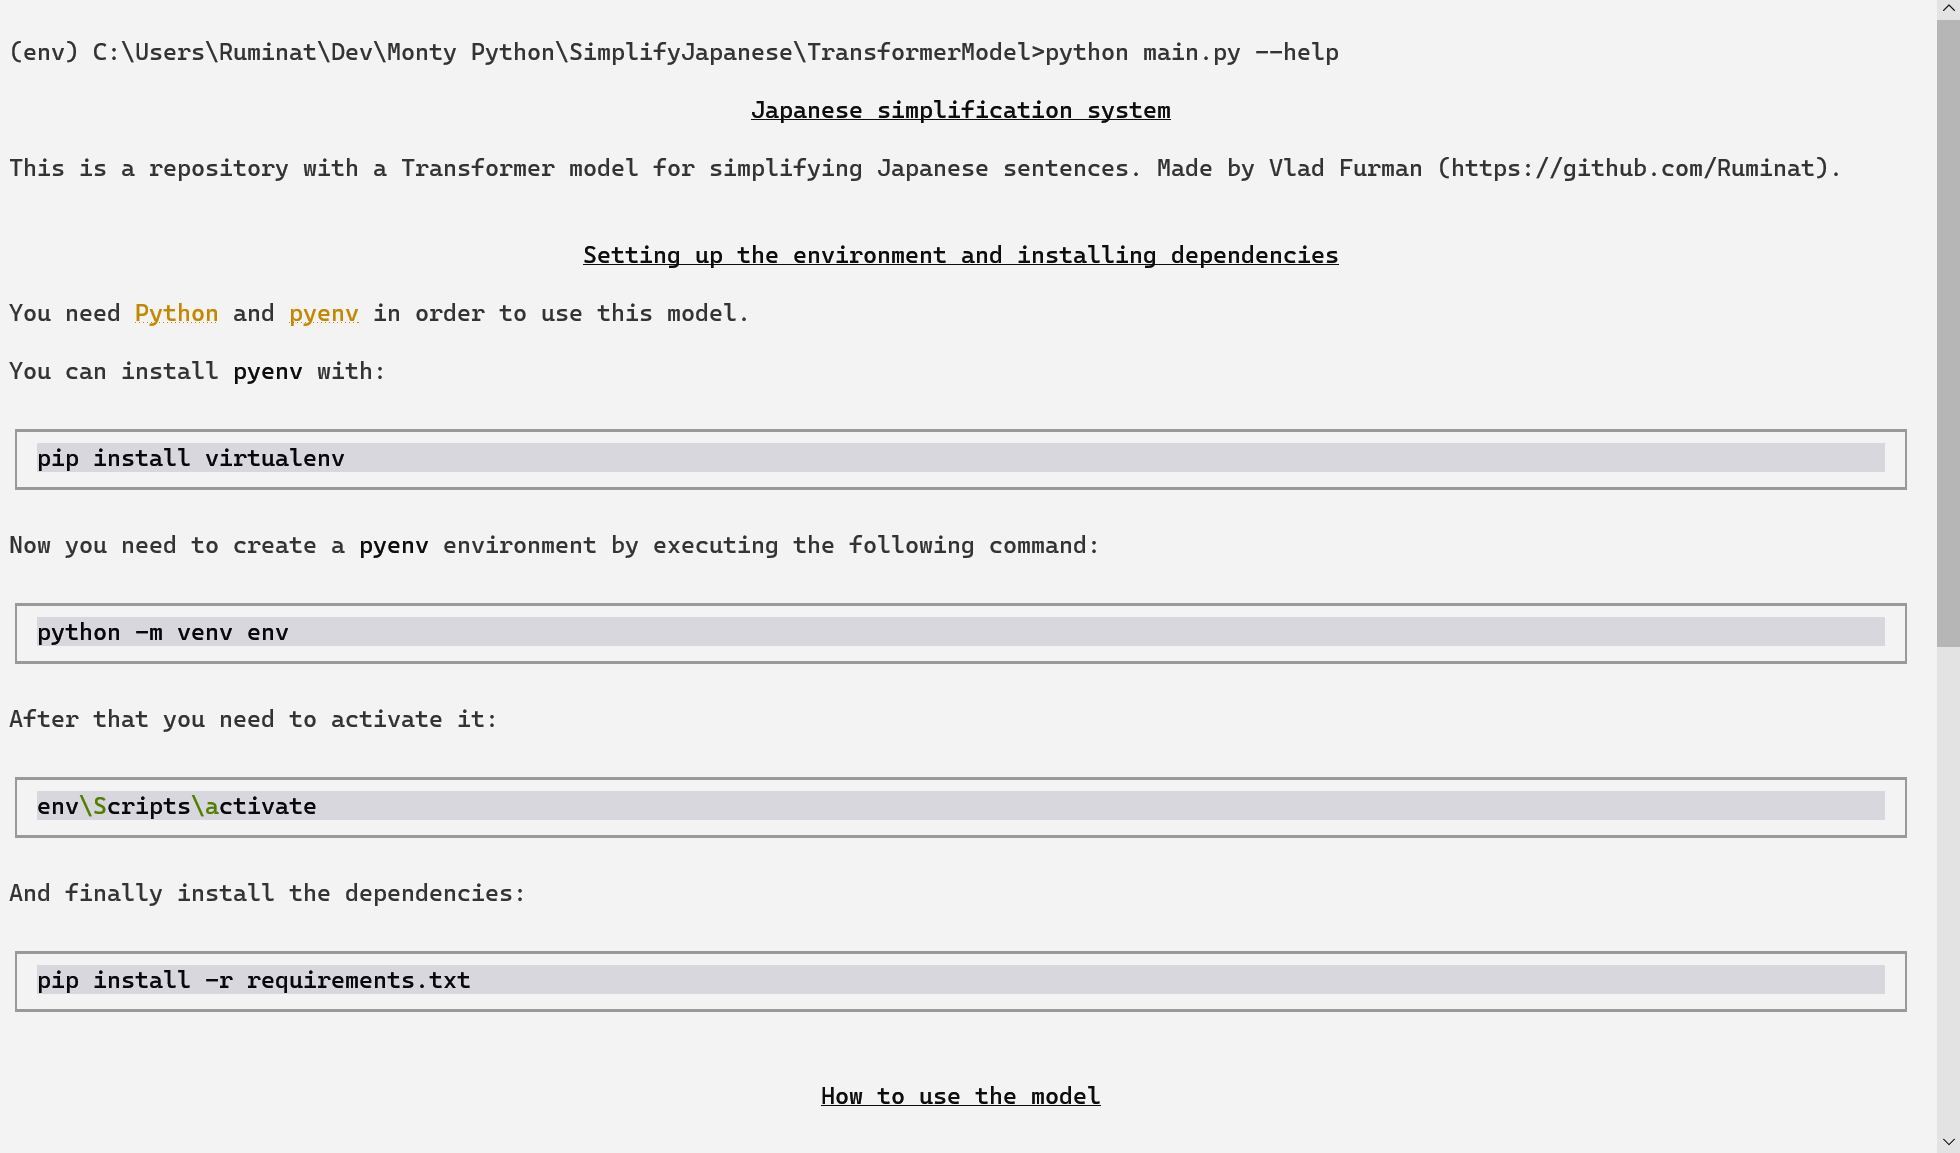
\includegraphics[width=\textwidth]{help.png}
  \caption{Частичный вывод команды \texttt{python main.py -{}-help}}
  \label{help}
\end{figure}

Поддерживаются также следующие флаги для команды \texttt{python main.py}:
\begin{enumerate}[1.]%
  \item \texttt{-{}-version} или просто \texttt{-{}-v} "--- выводит текущую версию системы,
  \item \texttt{-{}-no-print}  "--- отключает вывод упрощения тестовых предложений.
\end{enumerate}


% .---|||___|||--- S E C T I O N ---|||___|||---. %
\section{Сервер}
% .---|||___|||--- S E C T I O N ---|||___|||---. %


Как уже было сказано ранее, сервер использует фреймворк Falcon.
Имеется лишь один путь "--- \texttt{/processJapaneseText}, по которму пользовательское приложение передаёт запрос с японским текстом, после чего сервер, используя функции \texttt{getMeCabTokens}~и~\texttt{transformer.translate}, упрощает это предложение и возвращает результат приложению.


% .---|||___|||--- S U B S E C T I O N ---|||___|||---. %
\subsection{Настройка сервера}
% .---|||___|||--- S U B S E C T I O N ---|||___|||---. %


Чтобы использовать сервер, его необходимо сначала настроить.
Весь процесс подготовки окружения для сервера описан в \texttt{README.md} репозитория~\cite{ServerGithub}.
Нужно сделать следующее:
\begin{enumerate}[1.]%
  \item \texttt{pip install virtualenv} "--- установить virtual env,
  \item \texttt{python -m venv env} "--- создать virtual env,
  \item \texttt{env\textbackslash{}Scripts\textbackslash{}activate} "--- активировать virtual env,
  \item \texttt{pip install -r requirements.txt} "--- установить необходимые зависимости.
\end{enumerate}

Теперь сервер может быть запущен командами:
\begin{itemize}%
  \item \texttt{python main.py -{}-server} "--- в режиме разработки,
  \item \texttt{waitress-serve -{}-port=8000 server:app} "--- в production-окружении.
\end{itemize}


% .---|||___|||--- S U B S E C T I O N ---|||___|||---. %
\subsection{Как «общаться» с сервером}
% .---|||___|||--- S U B S E C T I O N ---|||___|||---. %


Как уже было сказано ранее, сервер имеет путь \texttt{/processJapaneseText}.
Вот пример запроса по этому пути через консольную утилиту \texttt{curl}: \\ 
\texttt{curl http://localhost:5000/processJapaneseText?text=\jp{お前はもう死んでいる}} \\ 
Пример ответа показан на~\firef{response}, где можно увидеть, что возвращается JSON со следующими полями:
\begin{itemize}%
  \item \texttt{originalText} "--- исходное предложение,
  \item \texttt{simplifiedText} "--- упрощённое предложение,
  \item \texttt{originalTextTokens} "--- исходные токены с частями речи,
  \item \texttt{simplifiedTextTokens} "--- упрощённые токены с частями речи.
\end{itemize}
\begin{figure}[H]%
  \centering
  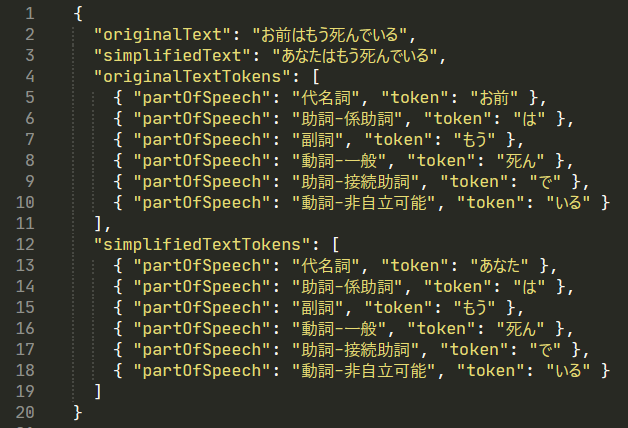
\includegraphics[height=8cm]{response.png}
  \caption{Пример ответа на запрос \texttt{/processJapaneseText}}
  \label{response}
\end{figure}


% .---|||___|||--- S E C T I O N ---|||___|||---. %
\section{Пользовательское приложение}
% .---|||___|||--- S E C T I O N ---|||___|||---. %


Пользовательское приложение выглядит довольно минималистично "--- есть форма ввода предложения, после нажатия на кнопку «Simplify» или нажатия «Ctrl»~+~«Enter» отправляется запрос на сервер (по пути \texttt{/processJapaneseText}), после чего ответ отображается в виде, как на~\firef{app-screen}.

Есть также возможность посмотреть перевод предложений (исходного и упрощённого) "--- при нажатии на ссылку «translation» открывается страница Google Translate с выбранным предложением "--- это может использоваться как некая опорная линия упрощения (что смысл не потерялся).

Цвета в предложениях (исходном и упрощённом) на~\firef{app-screen} указывают на часть речи какого-либо токена (слова).

\begin{figure}[H]%
  \centering
  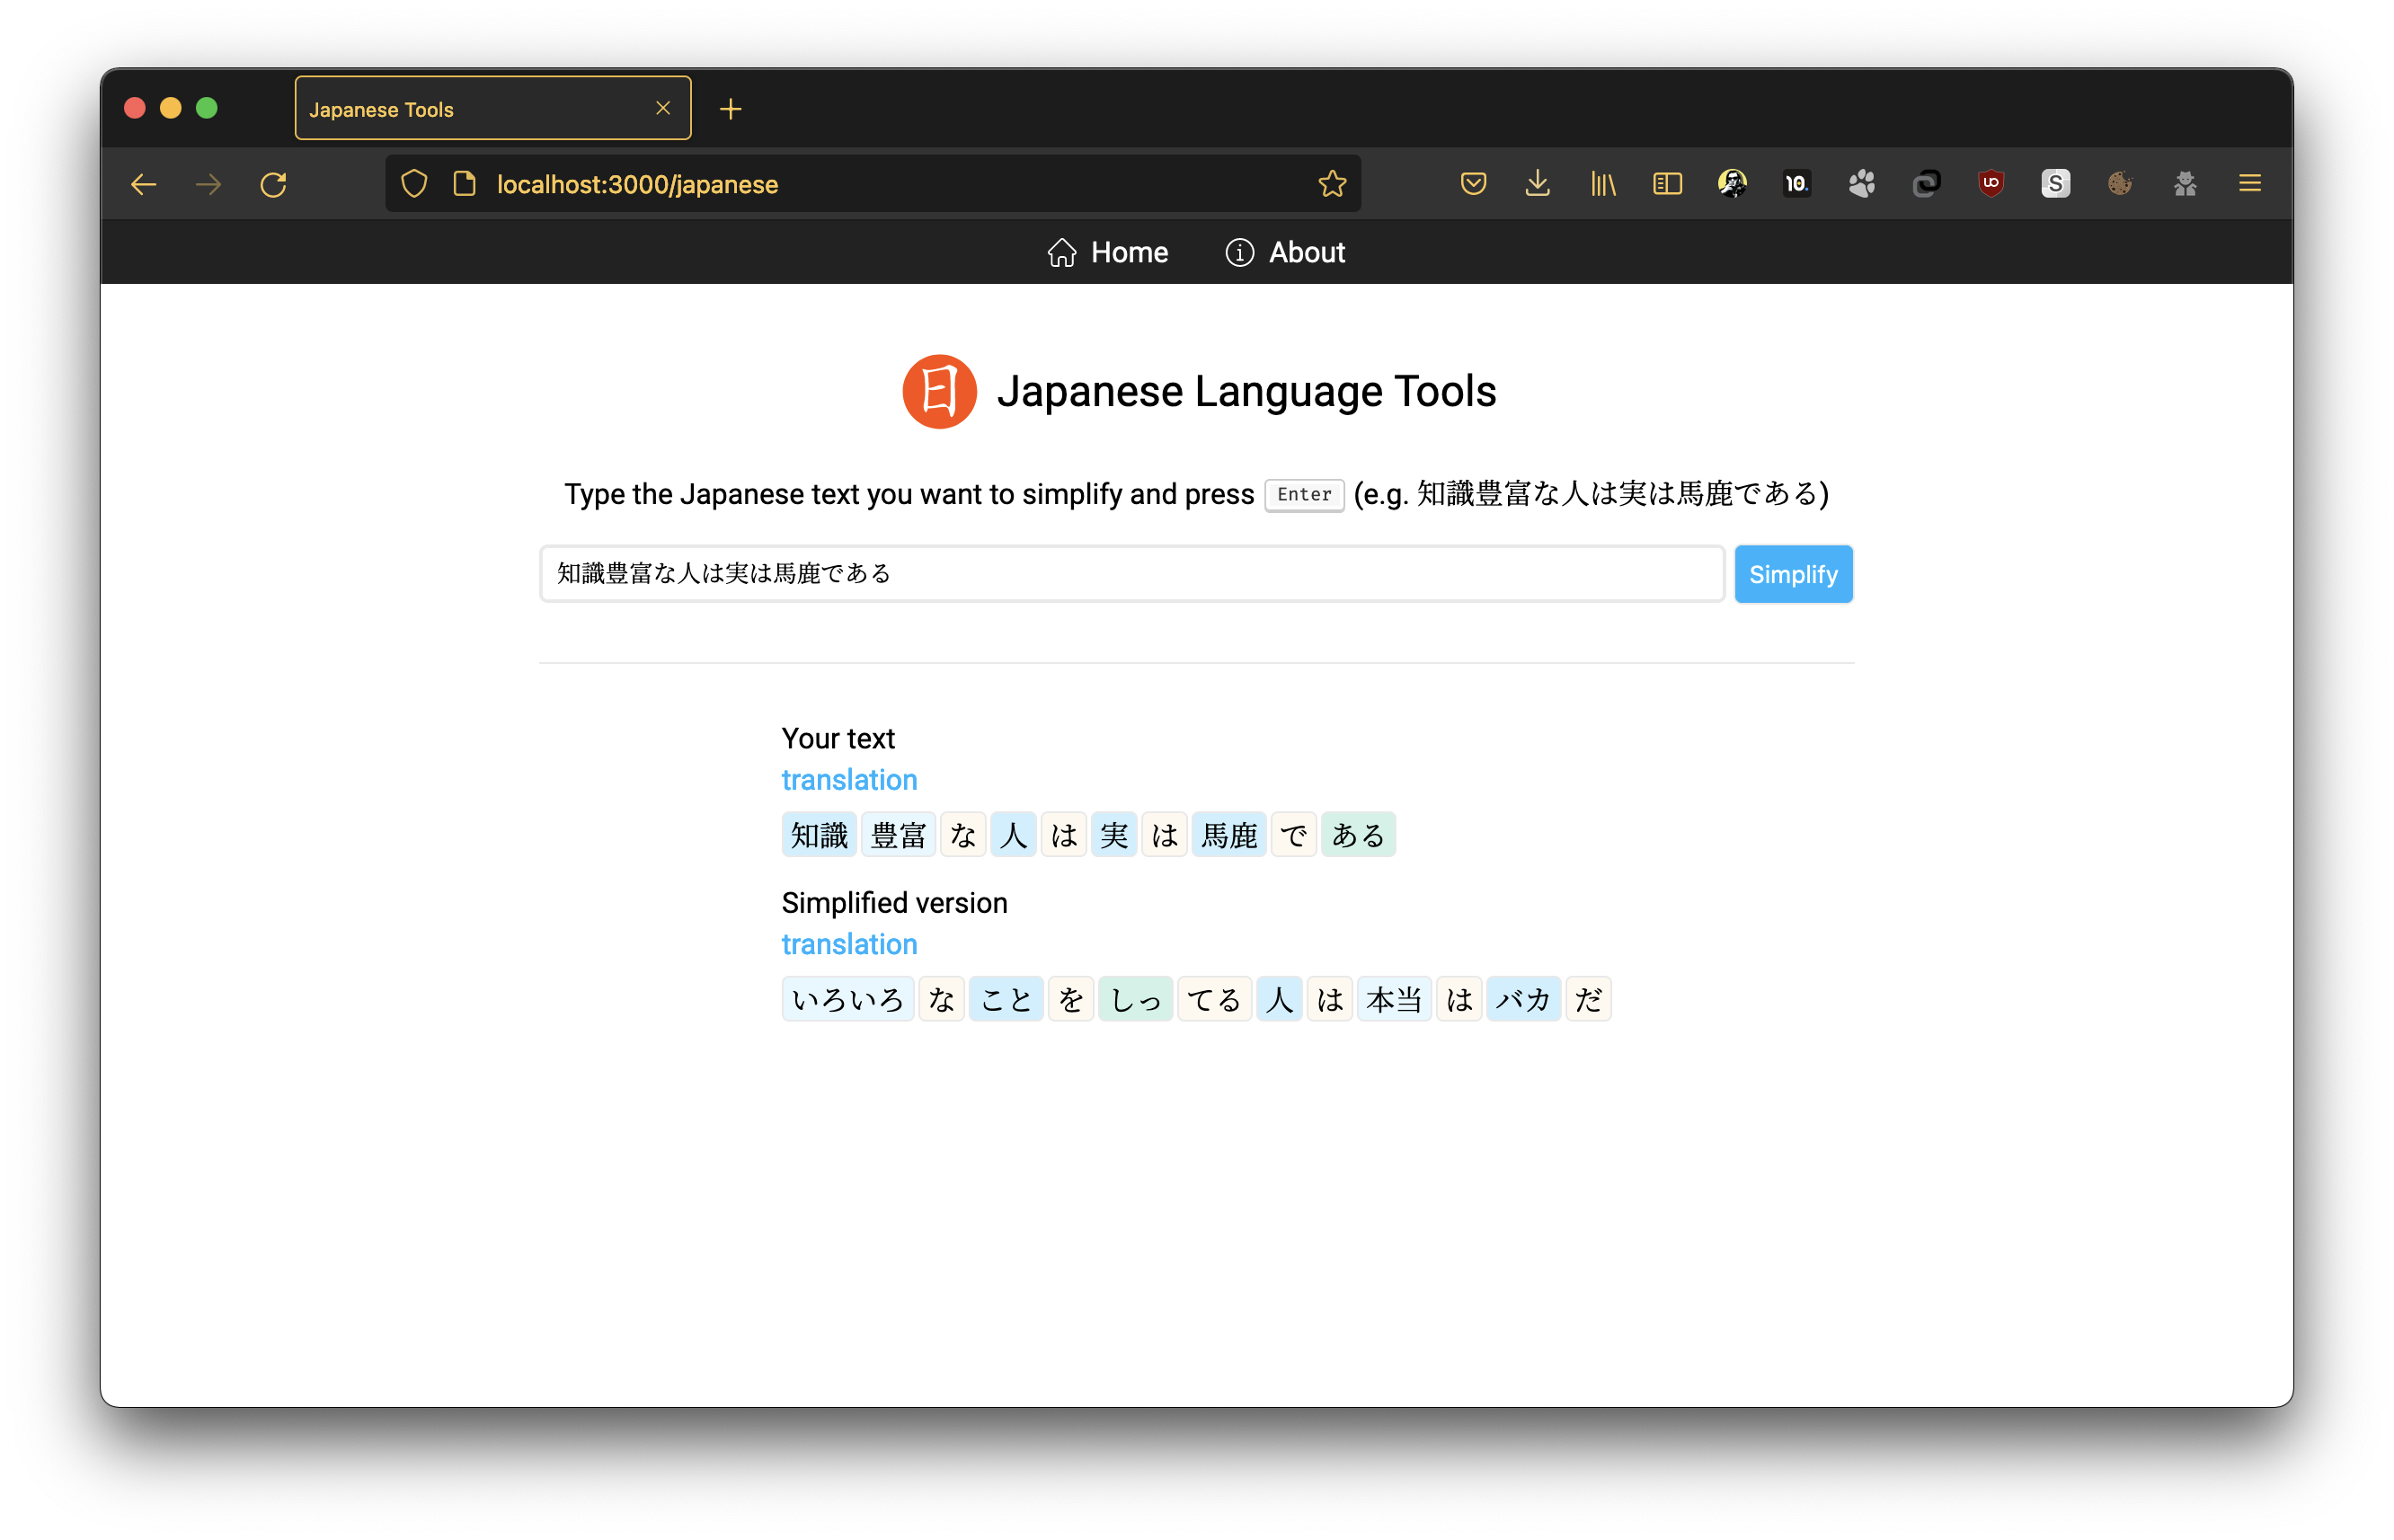
\includegraphics[width=\textwidth]{app.png}
  \caption{Пользовательское приложение}
  \label{app-screen}
\end{figure}
